% concours des contrats doctoraux EDMITT
\documentclass[table]{beamer}
\usepackage[utf8]{inputenc}
\usepackage[french]{babel}
\usepackage{wrapfig}
\usepackage{textpos}
\usepackage{listings}
\usepackage{xcolor}
\usepackage{fixltx2e} % textsubscript
%\usepackage{anyfontsize}
% User packages
\usepackage{lstlangarm}
\usepackage{ulem}
\usepackage{dsfont}

\usetheme{Warsaw}
\beamertemplatenavigationsymbolsempty
\setbeamertemplate{footline}[frame number]{}

\lstset{
    language=Caml,
    basicstyle=\ttfamily\scriptsize,
    keywordstyle=\color[rgb]{0.5,0,0}\bfseries,
    commentstyle=\color[rgb]{0.133,0.545,0.133},
    showstringspaces=false,
    frame=tb,
    columns=fullflexible,
    morekeywords={undefined}
}
\definecolor{Gray}{gray}{0.85}

\title{Détermination de propriétés de flots de données pour l'amélioration du temps d'exécution pire-cas}
\author{
    \emph{Candidat} \hspace{2.5cm} \emph{Encadrant}\\
    Jordy \textsc{Ruiz} \hspace{2.0cm} Hugues \textsc{Cassé}
}
\date{23 juin 2014}

\AtBeginSection[]
{
 \begin{frame}<beamer>
 \frametitle{Plan}
 \tableofcontents[currentsection]
 \end{frame}
}

\begin{document}
\frame{\titlepage}
\author{Jordy \textsc{Ruiz}}
\frame{\frametitle{Sommaire}\tableofcontents}

\section{Introduction}
\frame{\frametitle{Introduction}
	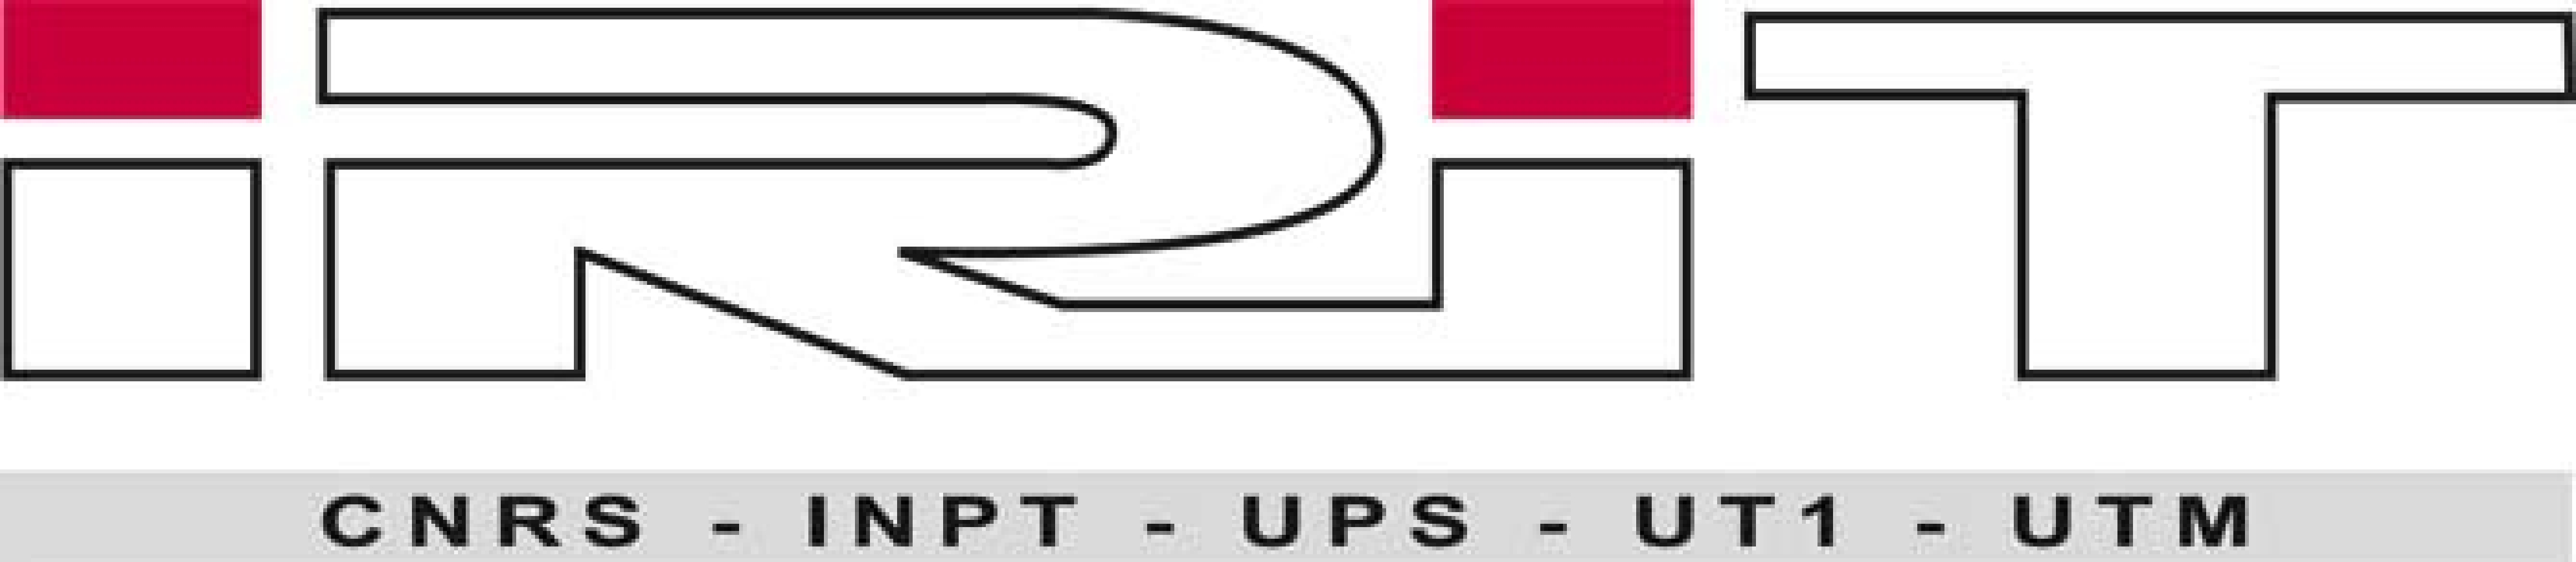
\includegraphics[height=30px]{pictures/logo_irit.jpg} \hfill
	
\includegraphics[height=30px]{pictures/otawa.png}
	
	\begin{center}
		\huge Équipe \textsc{traces}
	\end{center}
}

\section{Problématique et contexte}

\frame{\frametitle{Estimation du pire temps d'exécution (WCET)}
	\begin{itemize}[<+->]
		\item<1-> But : surestimer le temps d'exécution d'une partie de programme
		\item Exemples
		\begin{itemize}[<1->]
			\item Le frein de voiture s'activera au pire 50ms après la commande
			\item L'algorithme prendra une décision en moins d'1s
			\item ...
		\end{itemize}
		\item Systèmes temps-réel critiques : les mesures ne suffisent pas, il faut une \textbf{preuve} !
		\item Calcul du pire-temps : maximisation en ILP %% du système...
		\begin{itemize}[<1->]
			\item $\textit{WCET} = \max \sum x_i\; t_i$\\
			+ contraintes matérielles + contraintes logicielles
		\end{itemize}
	\end{itemize}
}


\frame{\frametitle{Recherche de chemins infaisables}
	\begin{columns}
		\begin{column}{.53\textwidth}
			\begin{itemize}[<+->]
				\item Graphe de flot de contrôle
				\item Chemins + SMT
				\begin{itemize}[<1->]
					\item $(x < 10) \wedge (x < 0)$
					\item $(x < 10) \wedge \neg (x < 0)$
					\item \textcolor{red}{$\neg (x < 10) \wedge (x < 0) \models \bot$}
					\item $\neg (x < 10) \wedge \neg (x < 0)$
				\end{itemize}
				\item Chemin infaisable\\ $\Rightarrow$ contrainte ILP\\
				$n_{(x < 0)} \leq n_{(x < 10)}$
			\end{itemize}
		\end{column}

		\begin{column}{.63\textwidth}
			\alt<1>{
			    \makebox[\textheight]{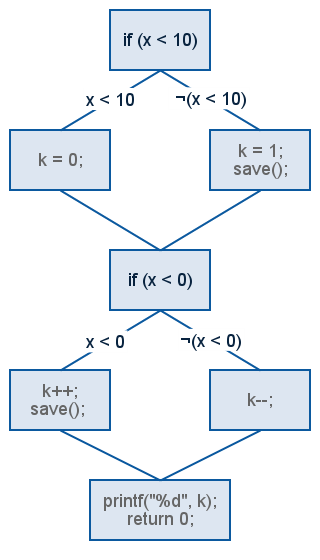
\includegraphics[height=210px]{pictures/cfg.png}}
			}{
			    \makebox[\textheight]{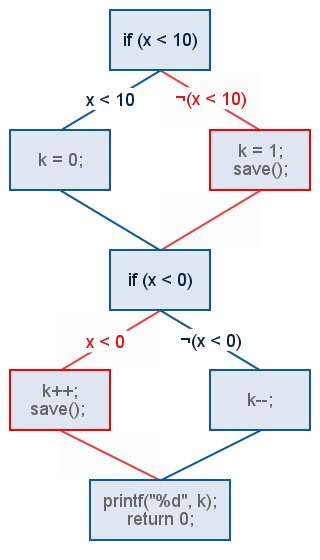
\includegraphics[height=210px]{pictures/cfg_infeasible.png}}
			}
		\end{column}
	\end{columns}
}

\frame{\frametitle{Choix du solveur SMT}
    \begin{wrapfigure}{r}{0in}
	
\includegraphics{pictures/cvc4.png}
    \end{wrapfigure}
    Notre choix de solveur s'est porté sur \textbf{CVC4} :

    \begin{itemize}
	\item Open-source, licence très libre
	\item De très bons résultats à la SMT-COMP
	\item Une API C++ riche et bien documentée
    \end{itemize}
}

\frame{\frametitle{Graphe en langage machine}
	\begin{center}
		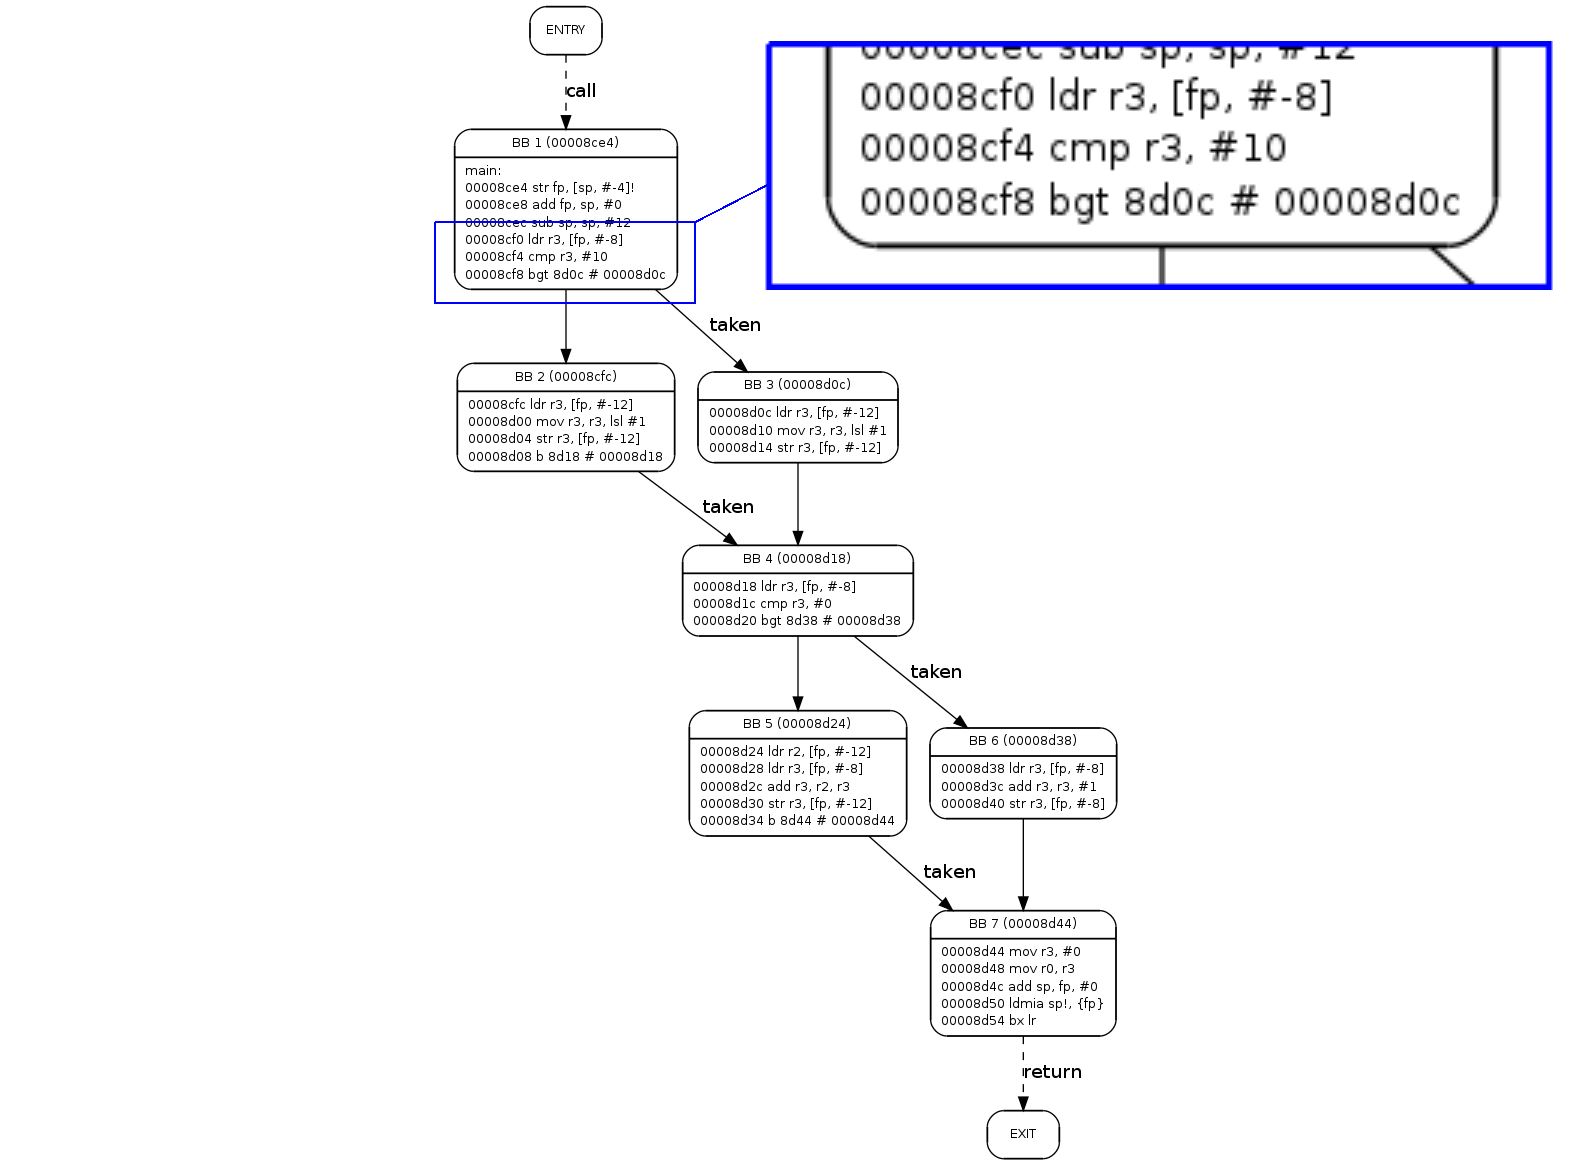
\includegraphics[height=0.9\textheight]{pictures/generated_cfg.png}
	\end{center}
}

\begin{frame}[fragile]
    \frametitle{Les instructions sémantiques d'OTAWA}
    \begin{minipage}{.36\linewidth}
	\begin{lstlisting}[language={[ARM]Assembler}]
	    ldr r0, [pc, #20]
	    @	seti ?15, 0x8310
	    @	seti t2, 0x14
	    @	add t1, ?15, t2
	    @	load ?0, t1, uint32

	    mov r1, #0
	    @	seti ?1, 0x0

	    mov r2, r1
	    @	set t1, ?1
	    @	set ?2, t1

	    bl 8574
	    @	seti t1, 0x8574
	    @	seti ?14, 0x8318
	    @	branch t1
	\end{lstlisting}
    \end{minipage}
    \begin{minipage}{.62\linewidth}
	Les variables d'OTAWA :

	\begin{itemize}
	    \item les registres machine \texttt{?0}, \texttt{?1}...(16, 32... ou plus selon l'architecture)
	    \item des variables temporaires \texttt{t1}, \texttt{t2}...
	    \begin{itemize}
		\item locales à une instruction machine (détruites à la fin)
		\item aident à la traduction en instructions sémantiques
	    \end{itemize}
	\end{itemize}
    \end{minipage}
\end{frame}

%\renewcommand\arraystretch{0.8} \setlength\minrowclearance{0.8pt}

% \begin{frame}[fragile]
%     \frametitle{Les instructions sémantiques d'OTAWA}
%     \begin{table} \tiny
% 	\begin{tabular}{|l|l|} \hline
% 	\textbf{Instruction} & \textbf{Sémantique}\\ \hline \hline
% 	\texttt{NOP} & (rien)\\ \hline
% 	\texttt{BRANCH, TRAP, CONT} & Indicateurs du flot du programme\\ \hline
% 	\texttt{IF cond sr jump} & si la condition \texttt{cond} sur le registre \texttt{sr} est vraie, continuer,\\
% 	& sinon sauter \texttt{jump} instructions\\ \hline
% 	\texttt{LOAD reg addr type} & reg $\leftarrow$ \texttt{MEM\textsubscript{type}} \\ \hline
% 	\texttt{STORE reg addr type} & \texttt{MEM\textsubscript{type}} $\leftarrow$ \texttt{reg}\\ \hline
% 	\texttt{SCRATCH d} & \texttt{d $\leftarrow$ $\top$} \textit{(invalidation)}\\ \hline
% 	\texttt{SET d a} & \texttt{d $\leftarrow$ a}\\ \hline
% 	\texttt{SETI d cst} & \texttt{d $\leftarrow$ cst}\\ \hline
% % 	\rowcolor{Gray} \texttt{SETP d cst} & \texttt{page(d) $\leftarrow$ cst}\\ \hline
% 	\texttt{CMP d a b} & \texttt{d $\leftarrow$ a $\sim$ b}\\ \hline
% 	\rowcolor{Gray} \texttt{CMPU d a b} & \texttt{d $\leftarrow$ a $\sim$\textsubscript{unsigned} b}\\ \hline
% 	\texttt{ADD d a b} & \texttt{d $\leftarrow$ a $+$ b}\\ \hline
% 	\texttt{SUB d a b} & \texttt{d $\leftarrow$ a $-$ b}\\ \hline
% 	\rowcolor{Gray} \texttt{SHL d a b} & \texttt{d $\leftarrow$ unsigned(a) <{<} b}\\ \hline
% 	\rowcolor{Gray} \texttt{SHR d a b} & \texttt{d $\leftarrow$ unsigned(a) >{>} b}\\ \hline
% 	\texttt{ASR d a b} & \texttt{d $\leftarrow$ a >{>} b}\\ \hline
% 	\texttt{NEG d a} & \texttt{d $\leftarrow$ $-$a}\\ \hline
% 	\rowcolor{Gray} \texttt{NOT d a} & \texttt{d $\leftarrow$ $\neg$a}\\ \hline
% 	\rowcolor{Gray} \texttt{AND d a b} & \texttt{d $\leftarrow$ a \& b}\\ \hline
% 	\rowcolor{Gray} \texttt{OR d a b} & \texttt{d $\leftarrow$ a | b}\\ \hline
% 	\rowcolor{Gray} \texttt{XOR d a b} & \texttt{d $\leftarrow$ a $\oplus$ b}\\ \hline
% 	\texttt{MUL d a b} & \texttt{d $\leftarrow$ a $\times$ b}\\ \hline
% 	\rowcolor{Gray} \texttt{MULU d a b} & \texttt{d $\leftarrow$ unsigned(a) $\times$ unsigned(b)}\\ \hline
% 	\texttt{DIV d a b} & \texttt{d $\leftarrow$ a / b}\\ \hline
% 	\rowcolor{Gray} \texttt{DIVU d a b} & \texttt{d $\leftarrow$ unsigned(a) / unsigned(b)}\\ \hline
% 	\texttt{MOD d a b} & \texttt{d $\leftarrow$ a \% b}\\ \hline
% 	\rowcolor{Gray} \texttt{MODU d a b} & \texttt{d $\leftarrow$ unsigned(a) \% unsigned(b)}\\ \hline
% % 	\rowcolor{Gray} \texttt{SPEC} & (instruction spéciale non supportée par OTAWA)\\ \hline
% 	\end{tabular}
%   \end{table}
% \end{frame}

\frame{\frametitle{Les instructions sémantiques d'OTAWA}
    \begin{itemize}%[<+->]
	\item Une trentaine d'instructions sémantiques
    \item On fait de l'analyse abstraite : on met à $\top$ quand on ne sait pas gérer\\
    \;$\Longrightarrow$ instruction \texttt{SCRATCH}\\
    \;$\Longrightarrow$ Il s'agit de toujours rester \textbf{correct}
    \end{itemize}
}


\section{Solution} % Algorithme de recherche de chemins infaisables
\frame{\frametitle{Représentation des prédicats}
    \begin{itemize}%
        \item \textbf{Prédicat} : Expression $\times$ Comparateur $\times$ Expression
        \item \textbf{Expression} :\\
        \qquad | Constante(k $\in \mathds{Z}$)\\
        \qquad | Variable(id $\in \mathds{Z}$)\\
        \qquad | Memoire(addr $\in \mathds{Z}$)\\[0.2cm]
        \qquad | ExprArithmétique
        \item \textbf{ExprArithmétique} : Expression $\times$ Operateur $\times$ Expression
    \end{itemize}
}

\frame{%\frametitle{}
	\begin{center}
		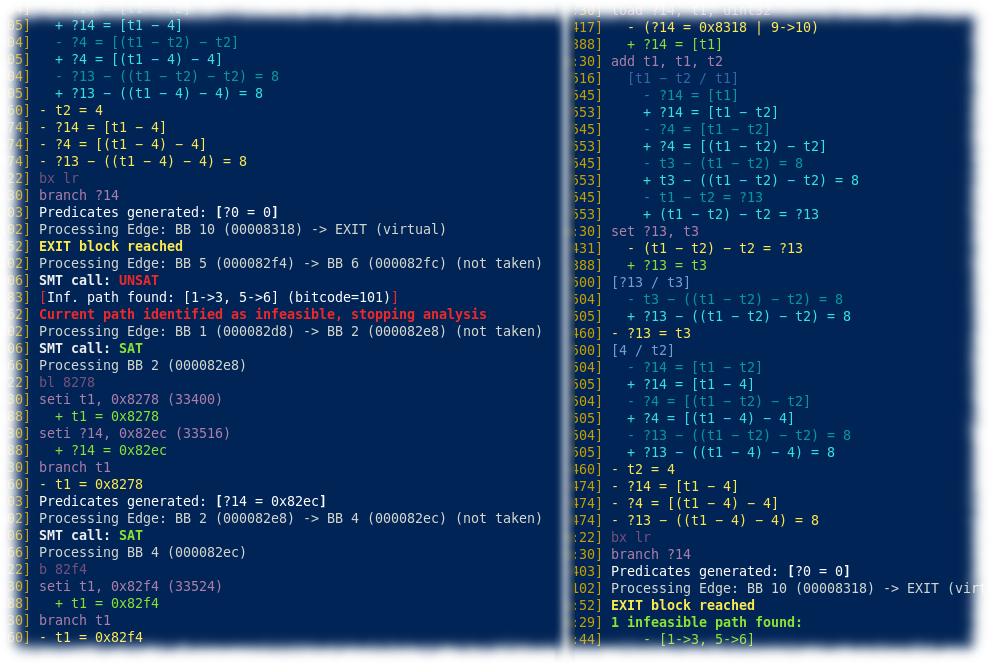
\includegraphics[height=0.75\paperheight]{pictures/pathfinder.png}
	\end{center}
}
\frame{%\frametitle{}
	\begin{center}
		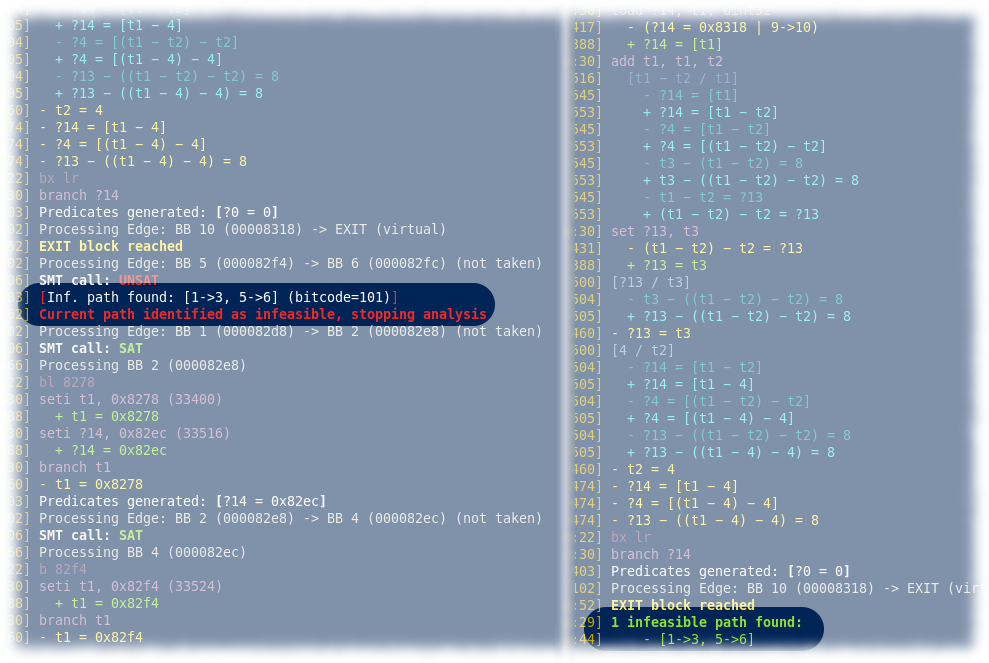
\includegraphics[height=0.75\paperheight]{pictures/pathfinder_goal.png}
	\end{center}
}
\frame{%\frametitle{}
	\begin{center}
		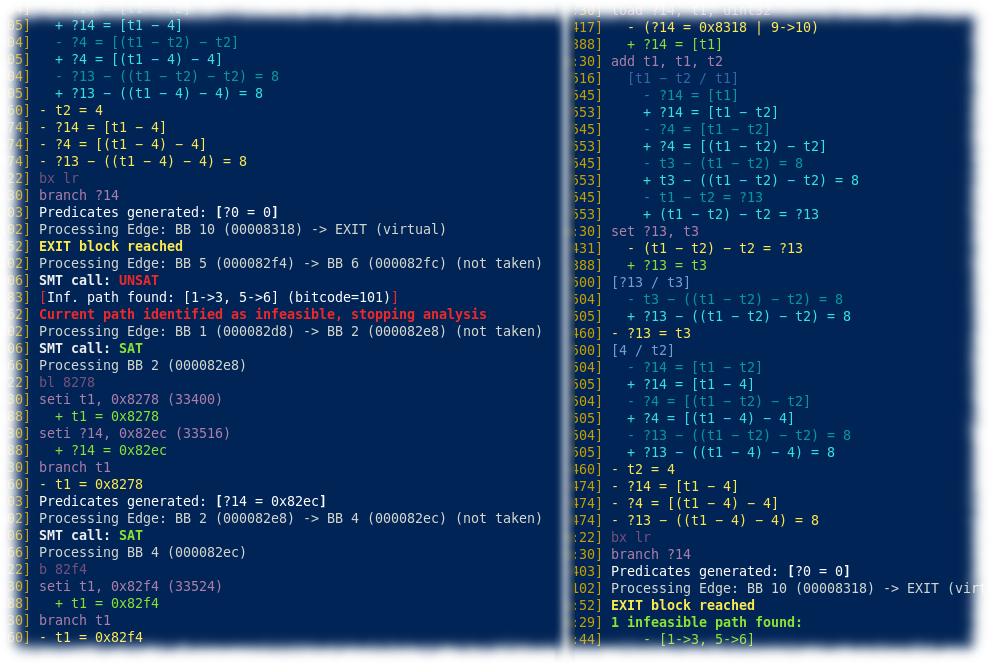
\includegraphics[height=0.75\paperheight]{pictures/pathfinder.png}
	\end{center}
}
\frame{%\frametitle{}
	\begin{center}
		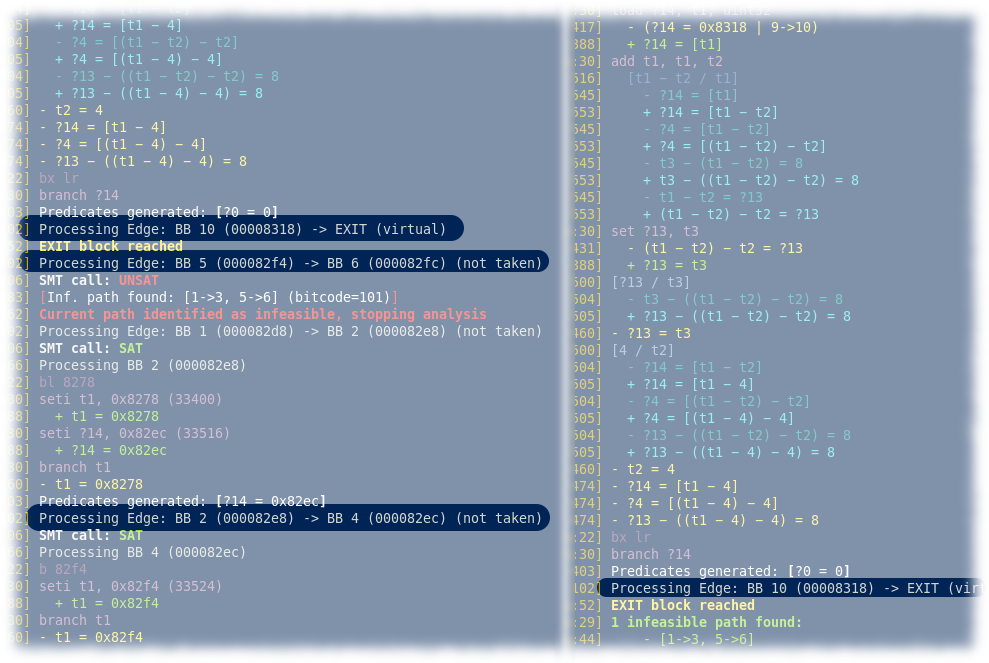
\includegraphics[height=0.75\paperheight]{pictures/pathfinder_edges.png}
	\end{center}
}
\frame{%\frametitle{}
	\begin{center}
		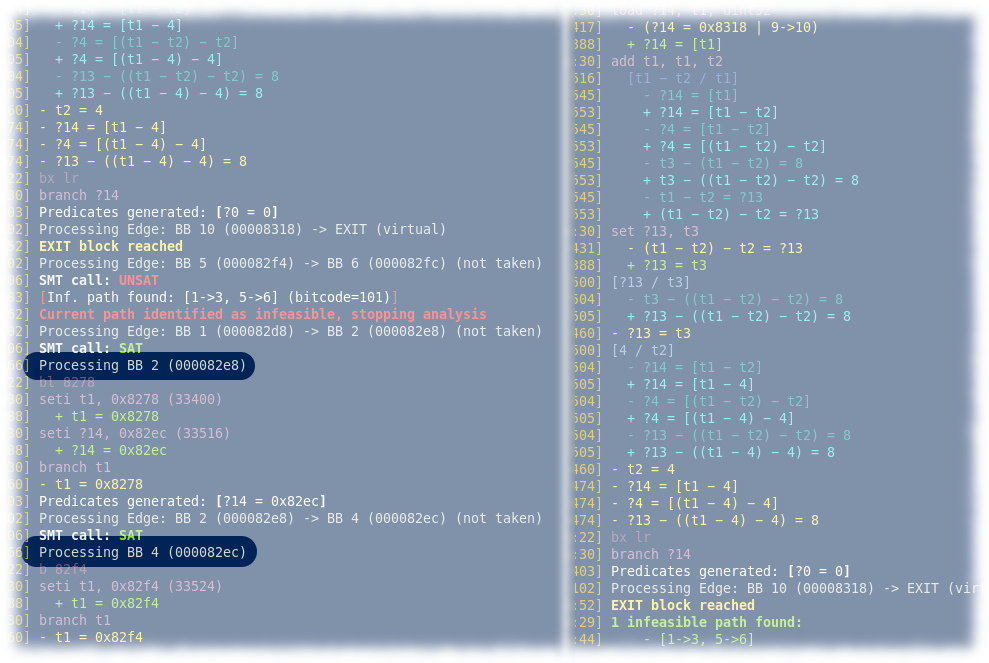
\includegraphics[height=0.75\paperheight]{pictures/pathfinder_bb.png}
	\end{center}
}
% \frame{%\frametitle{}
% 	\begin{center}
% 		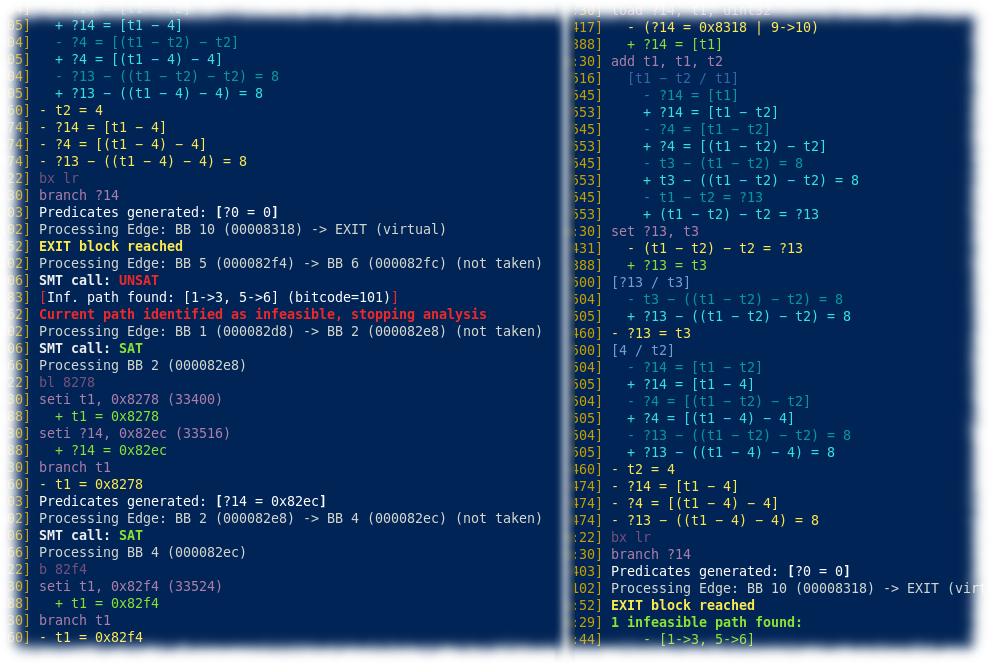
\includegraphics[height=0.75\paperheight]{pictures/pathfinder.png}
% 	\end{center}
% }
\frame{%\frametitle{}
	\begin{center}
		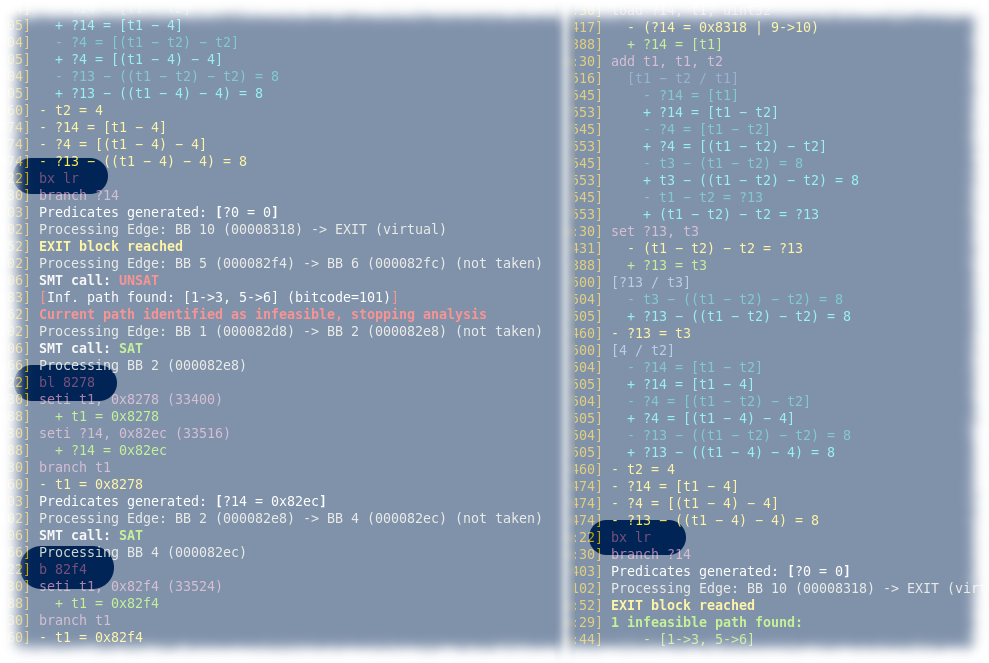
\includegraphics[height=0.75\paperheight]{pictures/pathfinder_arminst.png}
	\end{center}
}
\frame{%\frametitle{}
	\begin{center}
		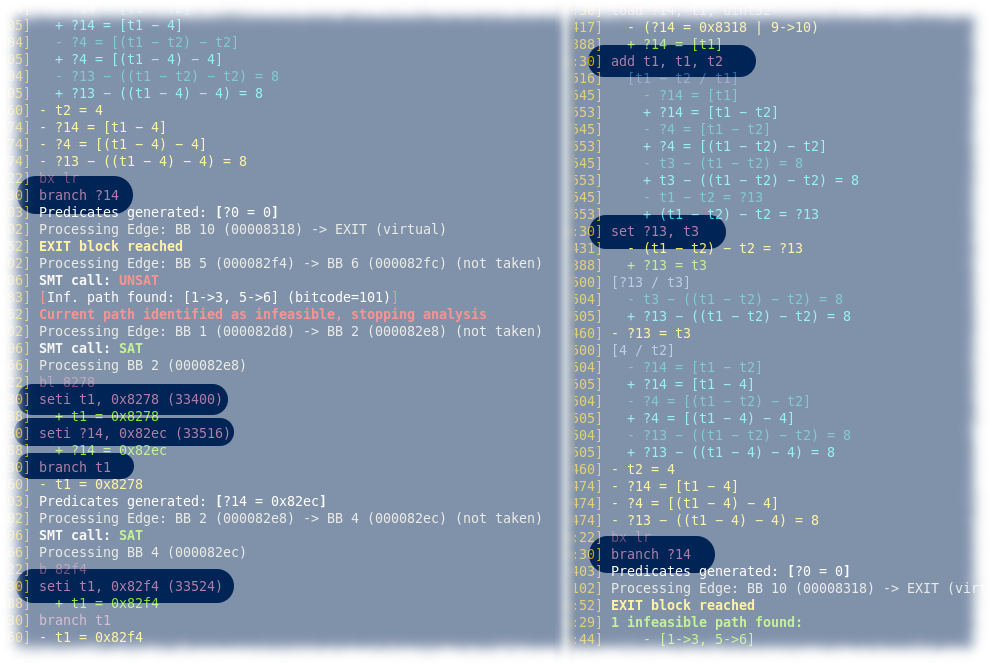
\includegraphics[height=0.75\paperheight]{pictures/pathfinder_seminst.png}
	\end{center}
}
\frame{%\frametitle{}
	\begin{center}
		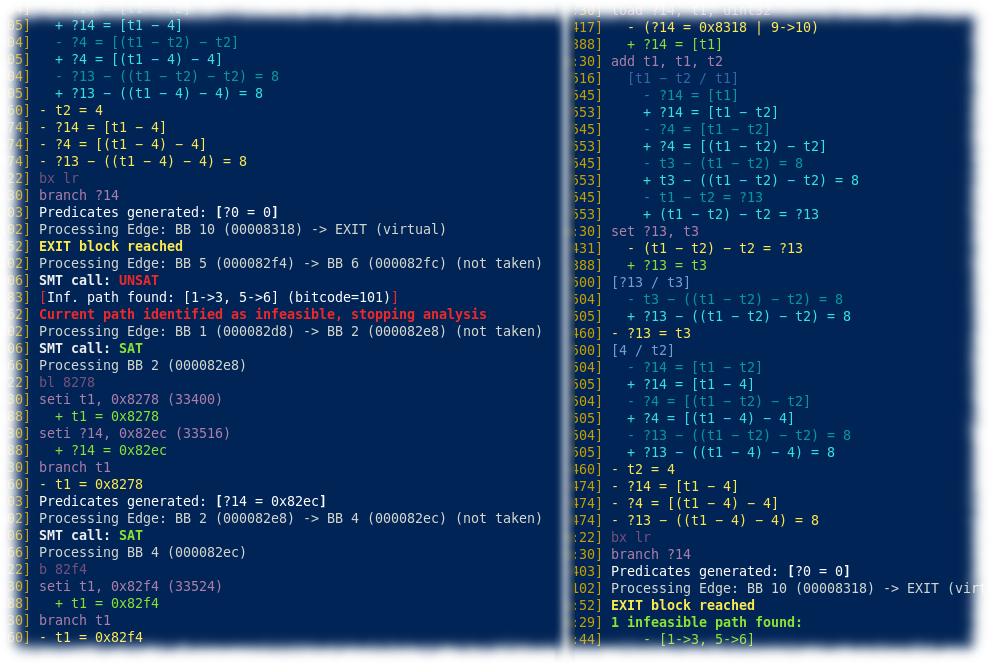
\includegraphics[height=0.75\paperheight]{pictures/pathfinder.png}
	\end{center}
}
\frame{%\frametitle{}
	\begin{center}
		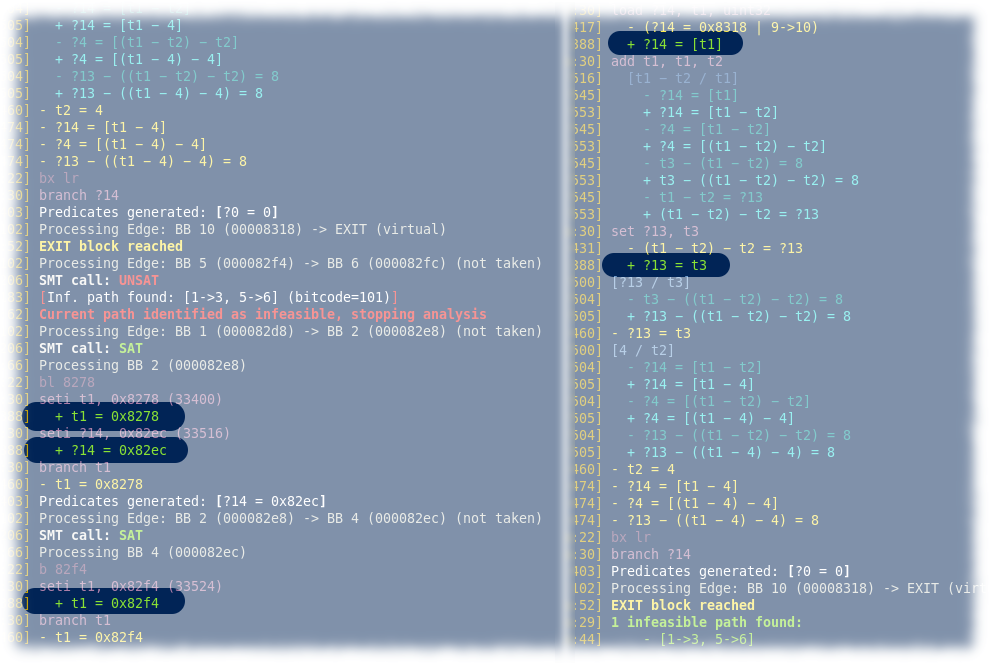
\includegraphics[height=0.75\paperheight]{pictures/pathfinder_preds_generated.png}
	\end{center}
}
\frame{%\frametitle{}
	\begin{center}
		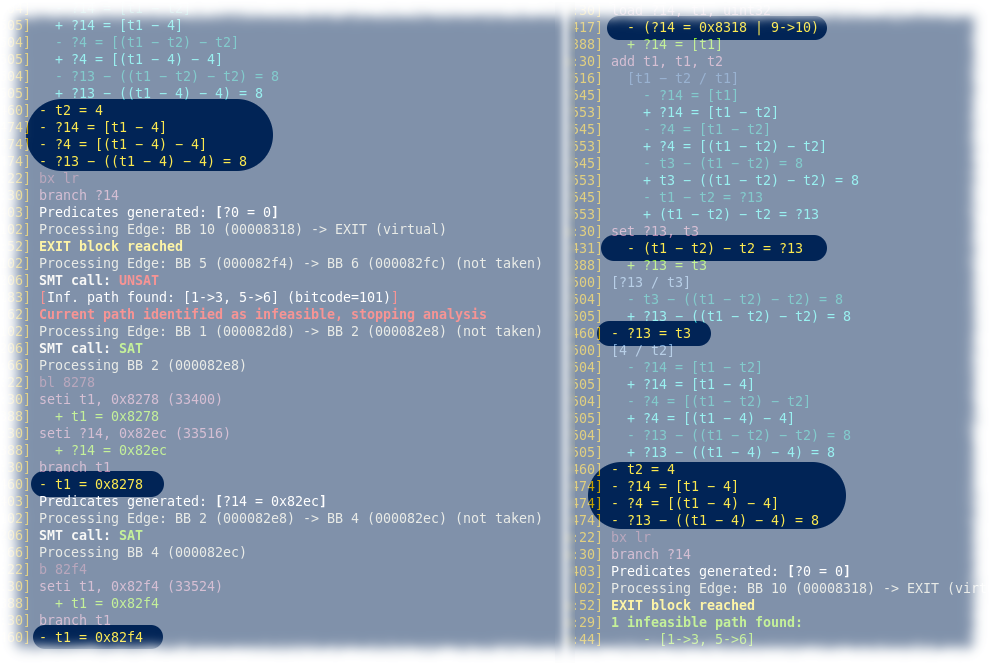
\includegraphics[height=0.75\paperheight]{pictures/pathfinder_preds_invalidated.png}
	\end{center}
}
\frame{%\frametitle{}
	\begin{center}
		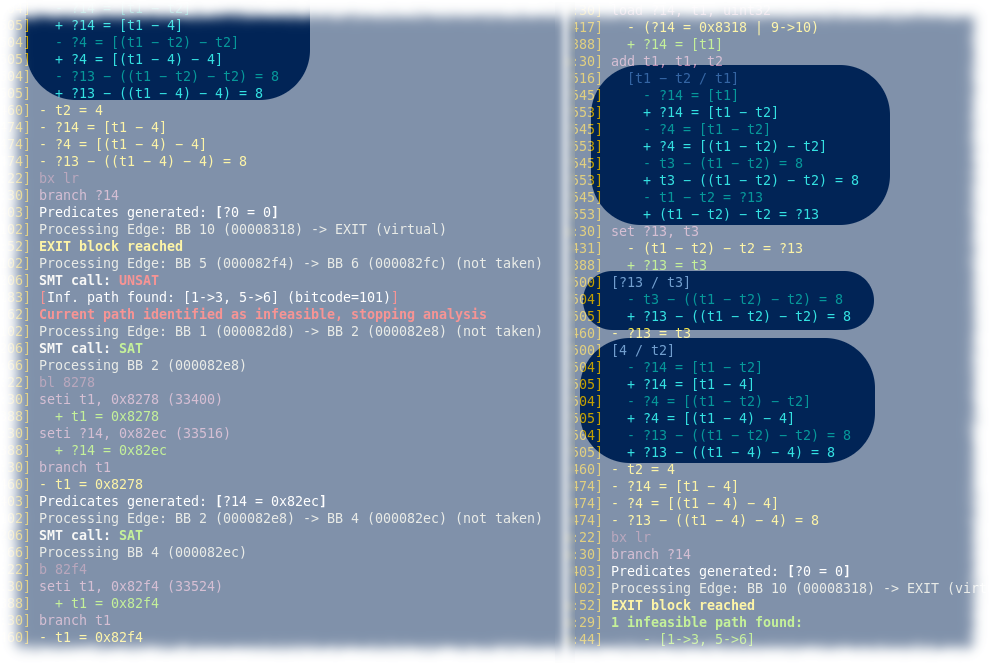
\includegraphics[height=0.75\paperheight]{pictures/pathfinder_preds_updated.png}
	\end{center}
}
\frame{%\frametitle{}
	\begin{center}
		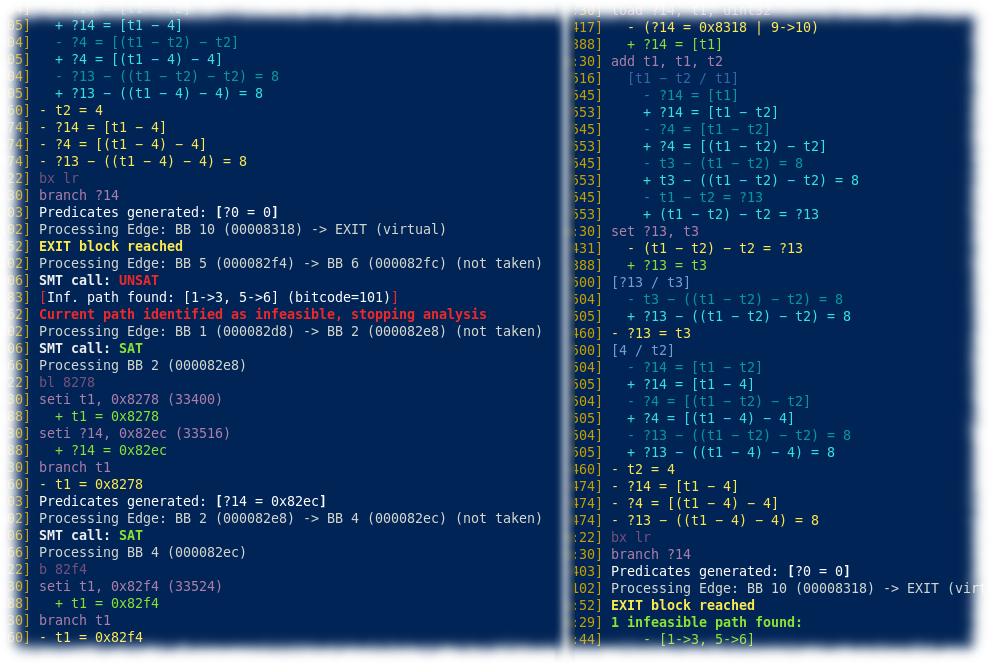
\includegraphics[height=0.75\paperheight]{pictures/pathfinder.png}
	\end{center}
}
\frame{%\frametitle{}
	\begin{center}
		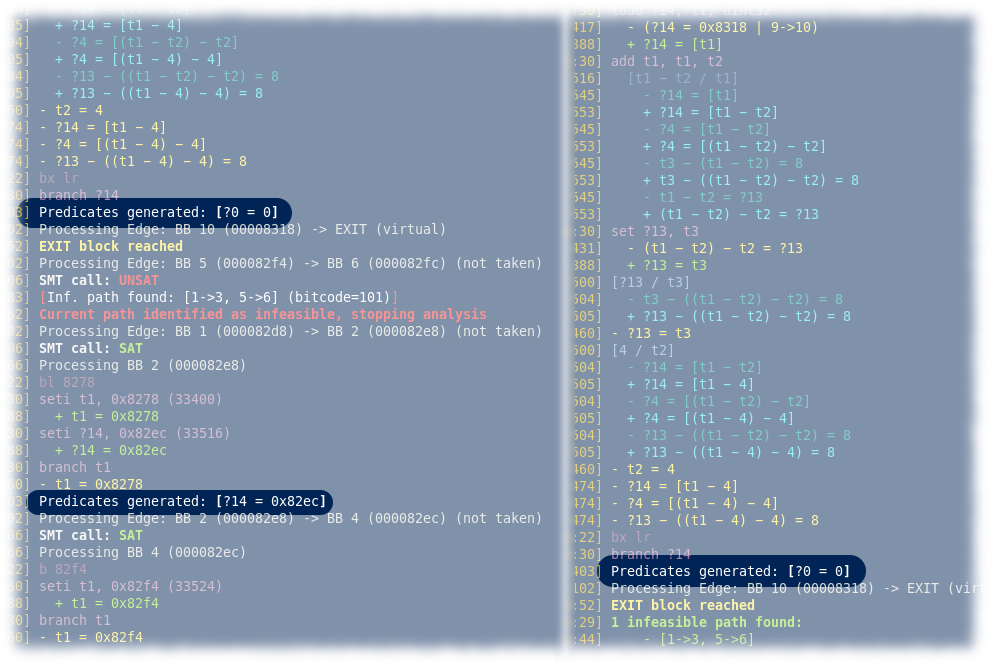
\includegraphics[height=0.75\paperheight]{pictures/pathfinder_end_bb_generated_preds.png}
	\end{center}
}
\frame{%\frametitle{}
	\begin{center}
		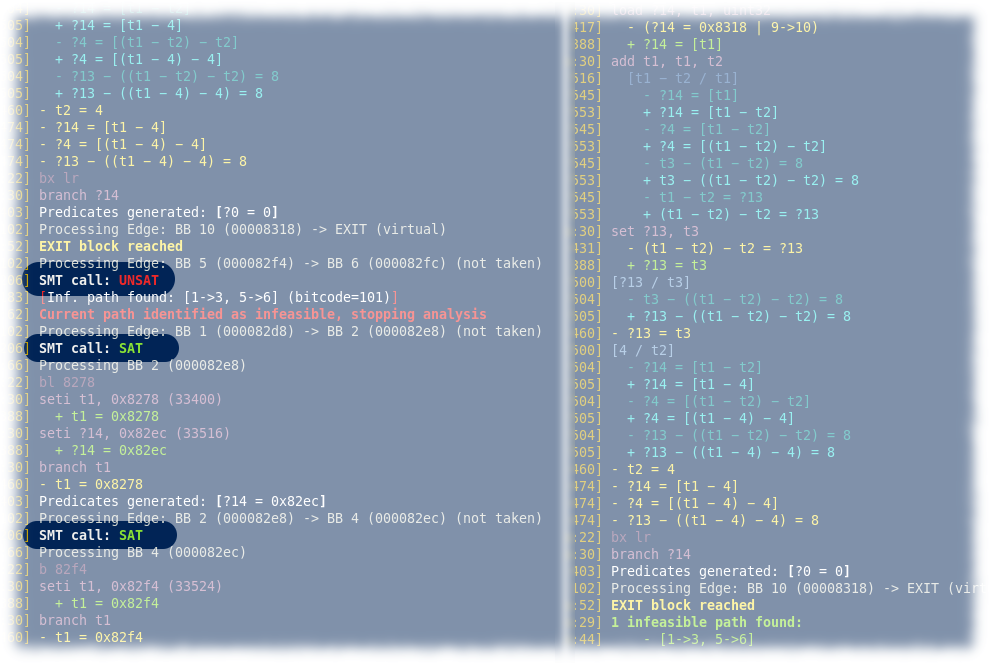
\includegraphics[height=0.75\paperheight]{pictures/pathfinder_smt_calls.png}
	\end{center}
}
%\frame{%\frametitle{}
%	\begin{center}
%		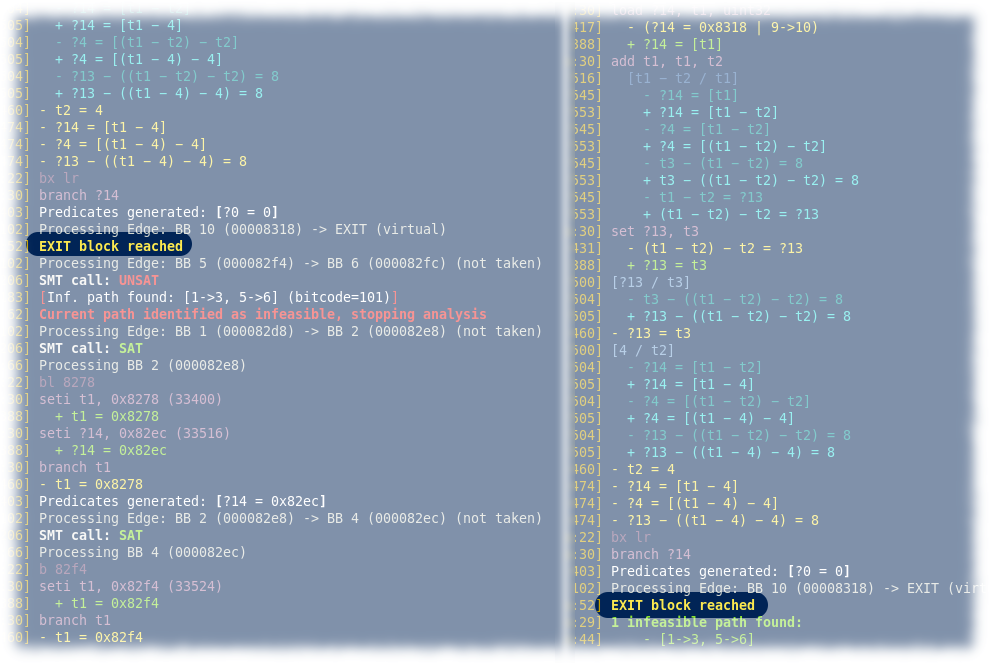
\includegraphics[height=0.75\paperheight]{pictures/pathfinder_exit.png}
%	\end{center}
%}
\frame{%\frametitle{}
	\begin{center}
		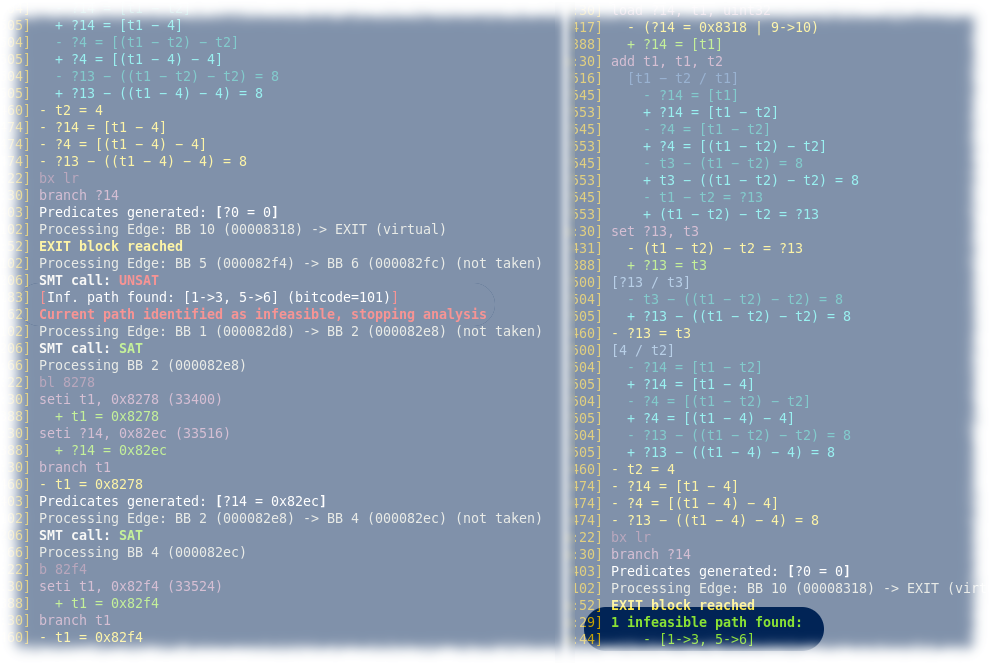
\includegraphics[height=0.75\paperheight]{pictures/pathfinder_result.png}
	\end{center}
}
\frame{%\frametitle{}
	\begin{center}
		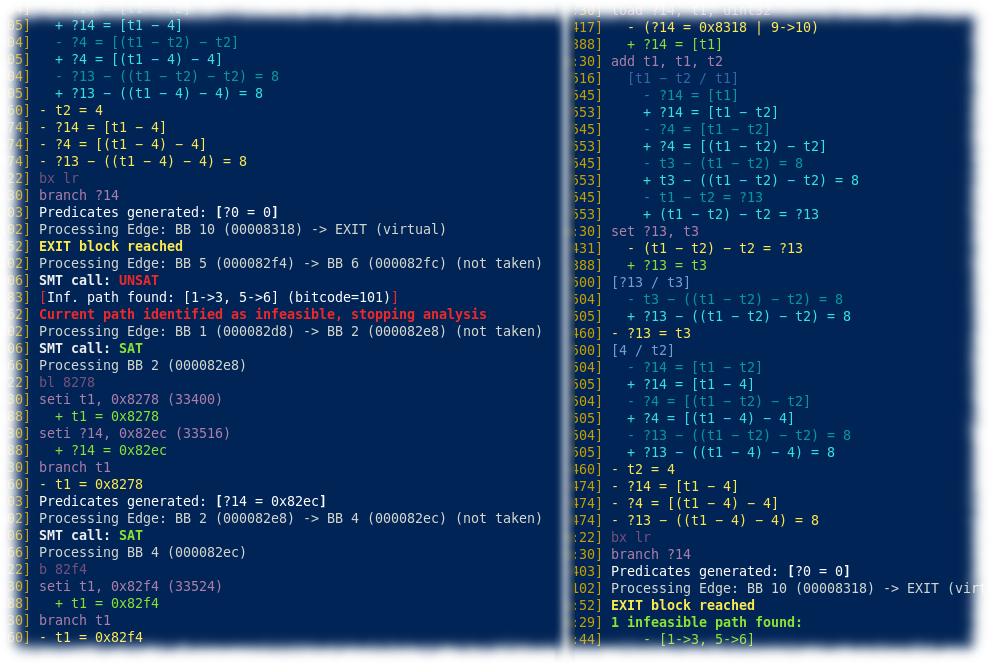
\includegraphics[height=0.75\paperheight]{pictures/pathfinder.png}
	\end{center}
}

\section{Ouvertures et conclusion}
\frame{\frametitle{Extensions}
	\begin{textblock*}{\textwidth}(0cm,-2cm)
		\begin{itemize}
			\item Thèse future dans la continuation du stage M2R, beaucoup d'extensions à faire :
			\begin{itemize}
				\item<2-> Traiter des programmes \textbf{avec boucles}\\
				$\Longrightarrow$ découpage du programme en partie sans boucles (ou avec boucles simples)
				\alt<2>{
					\vfill
					\begin{center}
						
\includegraphics{pictures/loop.png}
					\end{center}
				}{}
				\item<3-> Appels au solveur SMT plus intelligents
				\alt<3>{
					\end{itemize} \end{itemize}
					\vfill
					\begin{center}
						
\includegraphics{pictures/cvc4.png}
					\end{center}
					\begin{itemize} \item \begin{itemize}
				}{}
				\item<4-> Gérer les spécificités des types de données du langage machine % (spécificité de l'assembleur)
				\alt<4>{
					\end{itemize} \end{itemize}
					\vfill
					\begin{center}
						
\includegraphics{pictures/unsigned.png}
					\end{center}
					\begin{itemize} \item \begin{itemize}
				}{}
				\item<5-> Générer des contraintes ILP ne \textbf{suffit plus}\\
				$\Longrightarrow$ il faudrait faire de la \textbf{réécriture de graphe}.
			\end{itemize}
		\end{itemize}
	\end{textblock*}
}
\frame{\frametitle{Conclusion}
	\begin{itemize}[<+->]
		\item La recherche de chemins infaisables : un problème d'actualité
		\item A l'heure actuelle, on traite déjà certaines classes de programme
		\item Un travail qui trouve ses fondations dans l'interprétation abstraite
		\item \`A poursuivre en thèse...
	\end{itemize}
}

\usebackgroundtemplate{
\includegraphics[height=\paperheight]{pictures/questions.jpg}}
\frame{
    \begin{center}
        \huge{\textbf{Questions?}}
    \end{center}
}

\end{document}
